%-------------------------------------------------------------------------------
% seq64_rc_file
%-------------------------------------------------------------------------------
%
% \file        seq64_rc_file.tex
% \library     Documents
% \author      Chris Ahlstrom
% \date        2015-08-31
% \update      2017-03-19
% \version     $Revision$
% \license     $XPC_GPL_LICENSE$
%
%     Provides the rc_file.
%
%-------------------------------------------------------------------------------

\section{Sequencer64 "rc" Configuration File}
\label{sec:seq64_rc_file}

   \index{sequencer64.rc}
   \index{[sequencer64.rc]}   % for convenience
   The \textsl{Sequencer64} configuration file originally was \texttt{.seq24rc},
   and it was stored in the user's \texttt{\$HOME} directory.
   This is the same name used by \textsl{Seq24}, so we created an new file
   to take its place, with a fall-back to the original file-name if the new
   file does not exist, or if \textsl{Sequencer64} is running in
   \index{legacy mode}
   legacy mode.

   After you run \textsl{Sequencer64} for the first time (in non-legacy
   mode), it will generate a \texttt{sequencer64.rc} file in your home
   directory:

   \begin{verbatim}
      /home/ahlstrom/.config/sequencer64/sequencer64.rc
   \end{verbatim}

   It contains the the data for remote MIDI control, keyboard
   control, MIDI clock, and a few other settings.
   (See \sectionref{sec:seq64_usr_file} for some more settings.)

   \textsl{Sequencer64} will overwrite the \texttt{sequencer6.4rc} file upon
   quitting.  One should therefore quit \textsl{Sequencer64} before doing
   manual modifications to the \texttt{sequencer64.rc} file.

\subsection{Sequencer64 "rc" File / MIDI Control Section}
\label{subsec:seq64_rc_file_midi_control}

   Like \textsl{Seq24}, \textsl{Sequencer64} provides a way to control the
   application to some extent via a MIDI controller, such as a MIDI keyboard or
   a MIDI pad device.  The current section describes this feature;
   additional resources can be found at \url{linuxaudio.org}
   (\cite{midicontrol}).

   \index{[midi-control]}
   For each pattern, we can set up MIDI events to turn a 
	pattern on, off, or to toggle it.  This setup is in the 
   MIDI Control section of \texttt{sequencer64.rc}, and begins with an
   "INI-style" group marker \texttt{[midi-control]}.

% OR is it the current screen set and a set of mute groups???

   The MIDI control setup resembles a matrix.
   The matrix represents control for two functions of the active screen-set.
   These entries are numbered from 0 to 63.
   Legacy control keys occupy entries from 64 to 73.
   We've added some more entries, from 74 to 83, to control additional
   \textsl{Sequencer64} functions.
	
   The MIDI Control section is explicitly broken into subsections, though those
   subsections are marked with comment-lines for better comprehensibility.  The
   subsections of the MIDI Control section are:

   \begin{enumber}
      \item \textbf{Pattern group}.
         \index{rc!pattern group}
         Consists of 32 lines, one for each
         pattern box shown in the Pattern window.
         It provides a way to control the arming/disarming (muting/unmuting) of
         each pattern shown in the main window.  Note that the
         main window shows the \textsl{active} screen-set.  These controls affect
         the \textsl{active} screen-set.
      \item \textbf{Mute-in group}.
         \index{rc!mute-in group}
         Consists of 32 lines, one for each
         pattern box shown in the Pattern window.
         It provides a way to control the mute groups.
         A group is a set of sequences that can arm their playing state
         together; every group contains all 32 sequences in the
         \textsl{active} screen-set.
      \item \textbf{Automation group}.
         \index{rc!automation group}
         Each item in this group consists of one line.
         \begin{enumber}
            \item \textbf{bpm up}.
            \item \textbf{bpm down}.
            \item \textbf{screen-set up}.
            \item \textbf{screen-set down}.
            \item \textbf{mod replace}.
            \item \textbf{mod snapshot}.
            \item \textbf{mod queue}.
            \item \textbf{mod gmute}.
            \item \textbf{mod glearn}.
            \item \textbf{screen-set play}.
         \end{enumber}
      \item \textbf{Extended automation group}.
         \index{rc!extended automation}
         These additional control items were requested by users, to control
         addition features of the application.
         Each item in this group consists of one line.
         \begin{enumber}
            \item \textbf{stop/pause/start}.  Emulate the Stop, Pause, and
               Start keys, using Toggle for pause, Off for stop, and On for
               start.
            \item \textbf{record}.  For recording a live performance by
               recording the mute/unmute states that the musician played.
               Not yet functional.
            \item \textbf{solo on/off}.
               Not yet functional.
            \item \textbf{thru toggle}.
               Not yet functional.
            \item \textbf{reserved for expansion} (six of these are reserved).
         \end{enumber}
   \end{enumber}

   For all of these MIDI control lines,
   the three fields, each between the brackets, on each line, correspond to a
   \textsl{MIDI filter} to toggle, enable, or disable a sequence, change a
   selection, or activate a feature.
   If the incoming MIDI event value matches a value present in the filter, it
   will \textsl{toggle} (first field), \textsl{enable} (second field) or
   \textsl{disable} (third field) the sequence.

   We see the following lines in the MIDI Control section, which is broken
   into groups or subsections marked by comments:

   \begin{verbatim}
      [midi-control]
      74      # MIDI controls count

      # pattern group
       0  [0 0 0 0 0 0]   [0 0 0 0 0 0]   [0 0 0 0 0 0]            
       1  [0 0 0 0 0 0]   [0 0 0 0 0 0]   [0 0 0 0 0 0]          
       2  [0 0 0 0 0 0]   [0 0 0 0 0 0]   [0 0 0 0 0 0]   
      ...     ...            ...              ...
      31  [0 0 0 0 0 0]   [0 0 0 0 0 0]   [0 0 0 0 0 0]    

      # mute in group section:
      32  [0 0 0 0 0 0]   [0 0 0 0 0 0]   [0 0 0 0 0 0]   
      33  [0 0 0 0 0 0]   [0 0 0 0 0 0]   [0 0 0 0 0 0]   
      ...     ...            ...              ...
      63  [0 0 0 0 0 0]   [0 0 0 0 0 0]   [0 0 0 0 0 0]   

      # bpm up:
      64  [0 0 0 0 0 0]   [0 0 0 0 0 0]   [0 0 0 0 0 0]   
      # bpm down:
      65  [0 0 0 0 0 0]   [0 0 0 0 0 0]   [0 0 0 0 0 0]   
      # screen set up:
      66  [0 0 0 0 0 0]   [0 0 0 0 0 0]   [0 0 0 0 0 0]   
      # screen set down:
      67  [0 0 0 0 0 0]   [0 0 0 0 0 0]   [0 0 0 0 0 0]   
      # mod replace:
      68  [0 0 0 0 0 0]   [0 0 0 0 0 0]   [0 0 0 0 0 0]   
      # mod snapshot:
      69  [0 0 0 0 0 0]   [0 0 0 0 0 0]   [0 0 0 0 0 0]   
      # mod queue:
      70  [0 0 0 0 0 0]   [0 0 0 0 0 0]   [0 0 0 0 0 0]   
      # mod gmute:
      71  [0 0 0 0 0 0]   [0 0 0 0 0 0]   [0 0 0 0 0 0]   
      # mod glearn:
      72  [0 0 0 0 0 0]   [0 0 0 0 0 0]   [0 0 0 0 0 0]   
      # screen set play:
      73  [0 0 0 0 0 0]   [0 0 0 0 0 0]   [0 0 0 0 0 0]   
   \end{verbatim}

   The number (74) is the number of lines in the MIDI Control section.
   The new extended automation values bring this number up to 84:

   \begin{verbatim}
      # start playback:
      74  [0 0 0 0 0 0]   [0 0 0 0 0 0]   [0 0 0 0 0 0]
      # pause playback:
      75  [0 0 0 0 0 0]   [0 0 0 0 0 0]   [0 0 0 0 0 0]
      # stop playback:
      76  [0 0 0 0 0 0]   [0 0 0 0 0 0]   [0 0 0 0 0 0]
      # performance record:
      77  [0 0 0 0 0 0]   [0 0 0 0 0 0]   [0 0 0 0 0 0]
      # solo off:
      78  [0 0 0 0 0 0]   [0 0 0 0 0 0]   [0 0 0 0 0 0]
      # solo on:
      79  [0 0 0 0 0 0]   [0 0 0 0 0 0]   [0 0 0 0 0 0]
      # toggle THRU:
      80  [0 0 0 0 0 0]   [0 0 0 0 0 0]   [0 0 0 0 0 0]
      # reserved for expansion:
      81  [0 0 0 0 0 0]   [0 0 0 0 0 0]   [0 0 0 0 0 0]
      # reserved for expansion:
      82  [0 0 0 0 0 0]   [0 0 0 0 0 0]   [0 0 0 0 0 0]
      # reserved for expansion:
      83  [0 0 0 0 0 0]   [0 0 0 0 0 0]   [0 0 0 0 0 0]
   \end{verbatim}

   Not all of these new values are yet usable.  Currently, just the
   "start", "pause", and "stop" controls have been implemented.

   So let's concentrate on one line of data:

   \begin{verbatim}
      74  [0 0 0 0 0 0]   [0 0 0 0 0 0]   [0 0 0 0 0 0]
   \end{verbatim}

   The first number represents one of the following entities, depending on its
   value:

   \begin{itemize}
      \item \textbf{0 to 31}.  These items represent the \textbf{Pattern group}
         for patterns (sequences) 1 to 32.
      \item \textbf{32 to 63}.  These items represent the \textbf{Mute-in
         group} for patterns (sequences) 1 to 32.
      \item \textbf{64 to 73}.  These items represent the legacy \textsl{Seq24}
         controls, from \textbf{bpm up} to \textbf{screen set play}.
      \item \textbf{74 to 83}.  These items, if present, represent the
         new extended controls, to control addition playback features of
         \textsl{Sequencer64}.
   \end{itemize}
   
   Each set of brackets on the line corresponds to a "MIDI filter":

   \begin{itemize}
      \item The leftmost bracket set defines the \textsl{toggle} filter.
      \item The middle bracket set defines the \textsl{on} filter.
      \item The rightmost bracket set defines the \textsl{off} filter.
   \end{itemize}

   If the incoming MIDI event matches the filter, it will either
   \textbf{[toggle]}, \textbf{[on]}, or \textbf{[off]}
   the pattern/sequence, respectively.
   The layout of each filter inside the brackets is as follows:

      \textbf{[OPR INV STAT D1 D2min D2max]}

   \begin{itemize}
      \item \textbf{OPR} = \textbf{on/off}
      \item \textbf{INV} = \textbf{inverse}
      \item \textbf{STAT} = \textbf{MIDI status byte} (channel ignored) 
      \item \textbf{D1} = \textbf{data1}
      \item \textbf{D2min} = \textbf{data2 min}
      \item \textbf{D2max} = \textbf{data2 max}
   \end{itemize}

   If \textbf{OPR (on/off)} is set to 1, it will match the incoming MIDI
   against the \textbf{STAT (MIDI status byte)} pattern (with the channel
   nybble stripped off) and perform the action (on/off/toggle) if the data
   falls in the range specified.  All values are in decimal.

   The \textbf{INV (inverse)} field will make the pattern perform the opposite
   action (\textsl{off} for \textsl{on}, \textsl{on} for \textsl{off}) if the
   data falls outside the specified range.  This is cool because one can map
   several sequences to a knob or fader.

   The \textbf{STAT (MIDI status byte)} field is a MIDI status byte number in
   decimals.  The channel nybble of this byte is ignored.  One can look the
   possible status values up in the MIDI messages tables; the relevant data can
   be found at \cite{midicontroltable}.  As the channel on which the events are
   sent is ignored, it is sufficient to use the values for channel 1.  That is,
   0.

   The last three fields describe the range of data that will match.  The
   \textbf{D1 (data1)} field provides the actual MIDI event message number to
   detect, in decimal.  This item could be a Note On/Off event or a
   Control/Mode change event, for example.

   The \textbf{D2min (data2 min)} field is the minimum value of the event for
   the filter to match. For Note On/Off events, this would be the velocity
   value, for example.

   The \textbf{D2max (data2 max)} field is the maximum value of the event for
   the filter to match.

\subsubsection{Sequencer64 "rc" File / MIDI Control Pattern Group}
\label{subsubsec:seq64_rc_file_midi_control_pattern_group}

   Complex?  Here is an example for the some of the first 32 lines, which
   comprise the \textsl{pattern group}.
   The following is an example of responding
   to Note On events for note 0, with any velocity, to turn the pattern on,
   and Note Off events for note 0, and any velocity, to turn the pattern
   off.

   \begin{verbatim}
	          Toggle                 On                      Off
        1 [0 0 0 0 0 0]      [1 0  144 0 0 127]       [1 0 128 0 0 127]
   \end{verbatim}

   The first number, 1, indicates the second pattern (pattern numbering starts
   from 0).
   The first section, \textbf{Toggle}, is off (inactive).  All values are 0.
   There is no setup to use MIDI control to toggle pattern 1 here.
   
   On to the second section, \textbf{On}:

   \begin{itemize}
      \item The \textbf{On} section starts with \textbf{OPR} = 1,
         so it is on (1 = active).
      \item The \textbf{inverse} value is off (0 = inactive).
      \item The \textbf{MIDI status byte}, 144, which is 0x90 (hex), which
         is a Note On event on channel 0.  However, the channel is ignored.
      \item The \textbf{data1} values sets the actual Note value to 0,
         meaning the lowest possible MIDI note (pitch) value.
      \item \textbf{data2 min} value sets the minimum value to 0.
      \item \textbf{data2 max} sets the maximum value to 127.
   \end{itemize}

   Thus, receiving any Note On velocity for note 0 will turn sequence
   1 \textsl{on}.  This is the second pattern; in the default setup, key
   \texttt{q} would operate on this pattern as well.
   
   On to the \textbf{Off} section:

   \begin{itemize}
      \item The \textbf{Off} field is on (active).
      \item The \textbf{inverse} value is off (0 = inactive).
      \item The \textbf{MIDI status byte}, 128, which is 0x80 (hex), which
         128, which is 0x80 (hex), which is a Note Off event on channel 0.
      \item The \textbf{data1} values sets the actual Note value to 0,
         meaning the lowest possible MIDI note (pitch) value.
      \item \textbf{data2 min} value sets the minimum value to 0.
      \item \textbf{data2 max} sets the maximum value to 127.
   \end{itemize}

   Thus, receiving any Note Off velocity for note 0 will turn sequence
   1 \textsl{off}.

   So, basically, pattern 1 starts when any Note On for MIDI note 0
   is received, and it stops when any Note Off for MIDI note 0 is received.  
   One can easily extend this so that Note On/Off values from 0 to 31
   control the corresponding pattern slot.

   Obviously, one might not want Note On/Off events from any channel to trigger
   events, so some other event would likely be more useful.
   (Hmmmm, we could add an option to not strip the channel value....)

   The following example would map a row of sequences to one knob sending
   out changes for Control Code 1:

   \begin{verbatim}
	          Toggle                 On                      Off
        0 [0 0 0 0 0 0]      [1 1 176 1   0   15]     [0 0 0 0 0 0]
        1 [0 0 0 0 0 0]      [1 1 176 1  16   31]     [0 0 0 0 0 0]
        2 [0 0 0 0 0 0]      [1 1 176 1  32   47]     [0 0 0 0 0 0]
        3 [0 0 0 0 0 0]      [1 1 176 1  48   63]     [0 0 0 0 0 0]
        4 [0 0 0 0 0 0]      [1 1 176 1  64   79]     [0 0 0 0 0 0]
        5 [0 0 0 0 0 0]      [1 1 176 1  80   95]     [0 0 0 0 0 0]
        6 [0 0 0 0 0 0]      [1 1 176 1  96  111]     [0 0 0 0 0 0]
        7 [0 0 0 0 0 0]      [1 1 176 1 112  127]     [0 0 0 0 0 0]
   \end{verbatim}

   The \textbf{on} field is on (active).  Inverse is active.  The
   \textbf{MIDI status byte}, 176, is 0xB0 (hex), which is a Control Change
   event (channel ignored).  \textbf{data1} is 1, which is the controller
   number for a Modulation Wheel.  The \textbf{data2} ranges are set so
   that, as the controller data increases (as the modulation-wheel knob is
   turned, so to speak), patterns 0 through 7 come on one at a time until
   all are running.

   Here is another example from \cite{midicontrol}, which shows how to set up
   the "Sustain" control-change event to queue or un-queue a sequence:
   The \textsl{Akai MPK Mini} has a Sustain button and we can set the
   Sustain MIDI event (with MIDI status byte 176 [0xB0] to represent a
   Controller event, and control/mode change number 64 [0x40] to
   represent the Sustain or Pedal control) up as the queue modifier in
   the \texttt{mod queue} entry:

   \begin{verbatim}
   # mod queue
   #  [   toggle-filter       ] [      on-filter       ] [      off-filter   ]

   70 [0   0   0   0   0   0  ] [1   0   176 64 127 127] [1   0  176 64  0  0]

   #   OPR INV STA D1  mn mx     OPR INV STA D1 mn  mx   OPR INV STA D1  mn mx
   #                                      ^  ^                    ^  ^
   #                                      |  |                    |  |
   #                                      |   ----Sustain---------|--
   #                                       -------Control Change--
   \end{verbatim}

   So when the Sustain button is held down, and one presses one of the pads
   on the \textsl{MPK Mini}, the corresponding sequence gets queued.
   Here's a little table of the decimal numbers for some commonly-used MIDI
   controls:

   \begin{itemize}
      \item \textbf{128} or \textbf{129} for any Note On or Note Off events.
      \item \textbf{160} Polyphonic aftertouch.
      \item \textbf{176} Controller event.
      \item \textbf{192} Program change.
      \item \textbf{208} Aftertouch.
      \item \textbf{224} Pitch wheel.
   \end{itemize}

\subsubsection{Sequencer64 "rc" File / MIDI Control Mute In Group}
\label{subsubsec:seq64_rc_file_midi_control_mute_in_group}

   \index{mute-in group}
   \index{[midi-control]!mute-in group}
   This section controls 32 groups of mutes in the same way as 
	defined for \texttt{[midi-control]}, and is in fact placed in the
   \texttt{[midi-control]} section.
   A group is a set of patterns that can toggle their playing state
   together.  Every group contains all 32 sequences in the active screen set.
   So, this part of the MIDI Control section is used for muting and unmuting
   (and toggling) a group of patterns.

   What is the different between the \textbf{mute-in group}
   section and the \textbf{mute group} section?  The former defines the MIDI
   control values that can affect the muting of a group, while the latter
   specifies the armed patterns that are part of a group.

\subsubsection{Sequencer64 "rc" File / MIDI Control Automation Group}
\label{subsubsec:seq64_rc_file_midi_control_automation_group}

   \index{automation group}
   \index{[midi-control]!automation group}

   \setcounter{ItemCounter}{0}      % Reset the ItemCounter for this list.

   \itempar{bpm up}{[midi-control]!bpm up}
   Increases the BPM (speed) of the sequencer based on MIDI input.

   \itempar{bpm down}{[midi-control]!bpm down}
   Decreases the BPM (speed) of the sequencer based on MIDI input.

   \itempar{screen-set up}{[midi-control]!screen-set up}
   Increases the active screen-set of the sequencer based on MIDI input.

   \itempar{screen-set down}{[midi-control]!screen-set down}
   Decreases the active screen-set of the sequencer based on MIDI input.

   \itempar{mod replace}{[midi-control]!mod replace}
   This item provides a way to automate replacement.

   \itempar{mod snapshot}{[midi-control]!mod snapshot}
   This item provides a way to automate snapshots.

   \itempar{mod queue}{[midi-control]!mod queue}
   This item provides a way to automate queueing.

   \itempar{mod gmute}{[midi-control]!mod gmute}
   \index{group!muting}
   This item provides a way to automate group-muting.

   \itempar{mod glearn}{[midi-control]!mod glearn}
   \index{group!learning}
   This item provides a way to automate group-learning.

   \itempar{screen-set play}{[midi-control]!screen-set play}
   This item provides a way to automate screen set play.

\subsection{Sequencer64 "rc" File / MIDI Control Extended Automation Section}
\label{subsubsec:seq64_rc_file_midi_control_extended_automation_group}

   \index{rc!start/stop control}
   This section shows how to set up an extended automation control.

   Currently, this control is enabled only in the \textbf{wip} branch of the
   \textsl{Sequencer64} project, and the only extended control that works is
   the \textsl{stop/pause/start} functionality (which requires that the pause
   functionality be enabled at build time, which is the default).

   Here, we will set up \textsl{Sequencer64} so that the first three MIDI
   white keys (notes 0, 2, and 4) will become "Stop", "Pause", and "Start"
   buttons.

   The first step, if not already done, is to install the new version
   (\textbf{0.90.2 * wip} and above) of \textsl{Sequencer64},
   run it, and then exit.
   Verify in the regenerated "rc" file
   (\texttt{\textasciitilde/.config/sequencer64/sequencer64.rc}) that the
   following lines exist:

   \begin{verbatim}
      84      # MIDI controls count (74 or 84)
   \end{verbatim}

   and

   \begin{verbatim}
      # Extended MIDI controls:
      # start playback (pause, start, stop):
      74 [0 0   0   0   0   0] [0 0   0   0   0   0] [0 0   0   0   0   0]
   \end{verbatim}

   MIDI control 74's toggle/on/off sections will be used to implement the
   stop/pause/start functionality.  Replace the "74" line with the following
   line:

   \begin{verbatim}
      74 [1 0 144   2   0 127] [1 0 144   4   0 127] [1 0 144   0   0 127]
   \end{verbatim}

   This sets up MIDI Note On (144) values 2 (toggle/pause), 4 (on/start), and 0
   (off/stop).
   Now we are ready to test this feature.  One can use a MIDI keyboard to do
   so, but here we will use the \textsl{VMPK} (\cite{vmpk}) virtual MIDI
   piano keyboard application for this test.  Refer to the following figure.

\begin{figure}[H]
   \centering 
   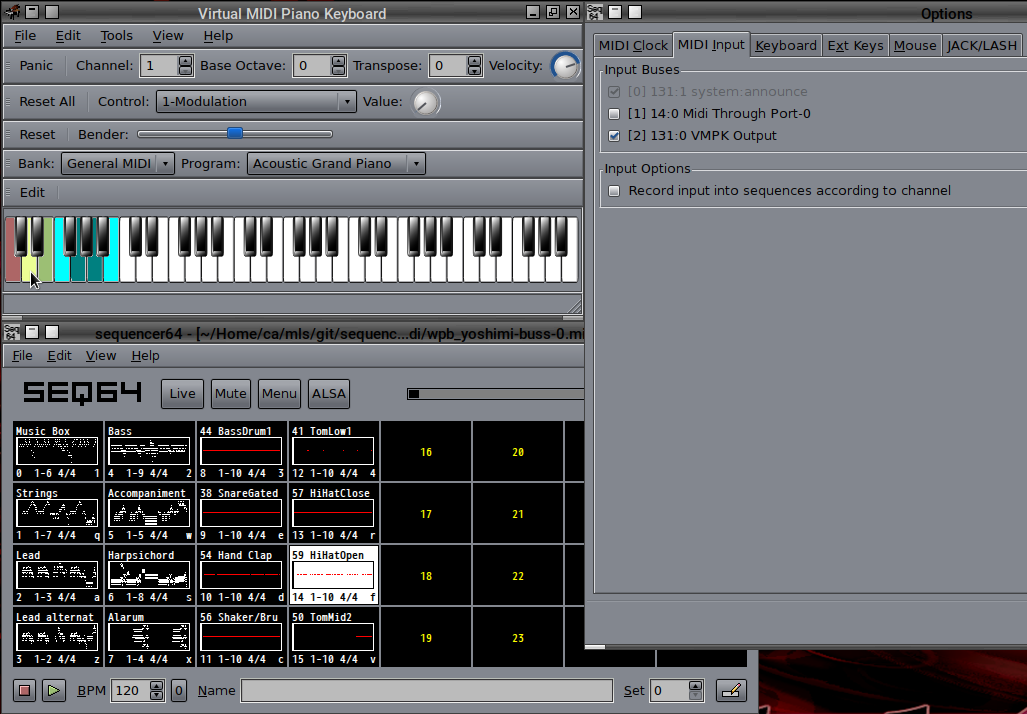
\includegraphics[scale=0.75]{new/stop_pause_start_test_setup.png}
   \caption{Stop/Pause/Start ALSA Test Setup}
   \label{fig:rc_file_stop_pause_start_alsa_test_setup}
\end{figure}

   Set up \textsl{VMPK} to use the lowest octave by setting
   \textbf{Base Octave} to \texttt{0}.  The red, yellow, and green
   keys shown will be our stop, pause, and start keys.

   Next, run \textsl{Sequencer64}, using the following command line to make
   sure that it is using ALSA and using automatic mode to connect the ALSA MID
   ports:

   \begin{verbatim}
      $ seq64 -A -a
   \end{verbatim}
   
   Then open a MIDI file.  Next,
   open the \textbf{File / Options / MIDI Input} tab, and make sure that
   the \textbf{VMPK Output} is check-marked as shown in the figure.
   If desired, also connect up to some kind of synthesizer so that the song can
   be heard.

   Finally, press the third white key (shown as green in the figure) to start
   playback.  The second white key (yellow in the figure) will pause and resume
   playback.  The first white key (red in the figure) will stop (and rewind)
   playback.

   Obviously, this setup is not useful for performance, but serves as a good
   example to verify this MIDI control.

   One thing we noticed while implementing this functionality is that there
   is really no need to have two lines for pairs such as BPM up/down and
   screen-set up/down.  Also, is screen-set play now partly redundant?
   No matter, we will not break the user's existing setup.

\subsection{Sequencer64 "rc" File / Mute-Group Section}
\label{subsec:seq64_rc_file_mute_group}
     
   This section is delimited by the \texttt{[mute-group]} construct.
   It controls 32 groups of mutes in the same way as defined for
   \texttt{[midi-control]}. A group is set of sequences that can toggle their
   playing state together.  Every group contains all 32 sequences in the
   active screen set.

   \begin{verbatim}
      [mute-group]
      1024    # group mute value count
      0 [0 0 0 0 0 0 0 0] [0 0 0 0 0 0 0 0] [0 0 0 0 0 0 0 0] [0 0 0 0 0 0 0 0]
      1 [0 0 0 0 0 0 0 0] [0 0 0 0 0 0 0 0] [0 0 0 0 0 0 0 0] [0 0 0 0 0 0 0 0]
      2 [0 0 0 0 0 0 0 0] [0 0 0 0 0 0 0 0] [0 0 0 0 0 0 0 0] [0 0 0 0 0 0 0 0]
      ...      ...               ...               ...               ...
      31 [0 0 0 0 0 0 0 0] [0 0 0 0 0 0 0 0] [0 0 0 0 0 0 0 0] [0 0 0 0 0 0 0 0]
   \end{verbatim}

   The initial number, 1024 is probably the total count of 32 x 32 sequences.
   In this group are the definitions of the state of the 32 sequences
   in the playing screen set when a group is selected.
   Each set of brackets defines a group:
   
   \begin{verbatim}
      [state of the first 8 sequences] [second 8] [third 8] [fourth 8]
   \end{verbatim}

   After the list of sequences and their MIDI events, one can 
   set \textsl{Sequencer64} to handle MIDI events and change some more settings
   in \texttt{sequencer64.rc}.

   What is the different between the \textbf{mute-in group}
   section and the \textbf{mute group} section?  The former defines the MIDI
   control values that can affect the muting of a group, while the latter
   specifies the patterns that are part of a group.

\subsection{Sequencer64 "rc" File / MIDI-Clock Section}
\label{subsec:seq64_rc_file_midi_clock}

   \index{[midi-clock]}
   The MIDI Clock fields will contain the clocking state from the last 
   time \textsl{Sequencer64} was run.  Turn off the clock with a 0, or on
   with a 1.
   This section has 16 entries, one for each MIDI output buss that
   \textsl{Sequencer64} supports.

   This configuration item is the same as the 
   \textbf{MIDI Clock} tab described in
   \paragraphref{paragraph:seq64_menu_file_options_midi_clock}
   
   Here is the format:

   \begin{verbatim}
      [midi-clock]
      16
       0 0  #  [1] seq24 1
       1 0  #  [2] seq24 2
       2 0  #  [3] seq24 3
       3 0  #  [4] seq24 4
       4 0  #  [5] seq24 5
       5 0  #  [6] seq24 6
       6 0  #  [7] seq24 7
       7 0  #  [8] seq24 8
       8 0  #  [9] seq24 9
       9 0  # [10] seq24 10
      10 0  # [11] seq24 11
      11 0  # [12] seq24 12
      12 0  # [13] seq24 13
      13 0  # [14] seq24 14
      14 0  # [15] seq24 15
      15 0  # [16] seq24 16
   \end{verbatim}

   That sample would be written one had started up \textsl{Sequencer64} in
   manual-alsa-mode.  On our system, where we have Timidity running, and
   erroneously have also specified 3 MIDI busses that we do not have, in the
   \texttt{sequencer64.usr} file:

   \begin{verbatim}
      [midi-clock]
      5    # number of MIDI clocks/busses
      # Output buss name: [0] 14:0 2x2 A (SuperNova,Q,TX81Z,DrumStation)
      0 0  # buss number, clock status
      # Output buss name: [1] 128:0 2x2 B (WaveStation,ESI-2000,MV4,ES-1,ER-1)
      1 0  # buss number, clock status
      # Output buss name: [2] 128:1 PCR-30 (303)
      2 0  # buss number, clock status
      # Output buss name: [3] 128:2 TiMidity port 2
      3 0  # buss number, clock status
      # Output buss name: [4] 128:3 TiMidity port 3
      4 0  # buss number, clock status
   \end{verbatim}

\subsection{Sequencer64 "rc" File / Keyboard Control Section}
\label{subsec:seq64_rc_file_keyboard_control}
        
   \index{[keyboard control]}
   The keyboard control is a dump of the keys that \textsl{Sequencer64}
   recognises, and each key's corresponding sequence number.
   Note that the first number corresponds to the number of sequences in
   the active screen set.

   \begin{verbatim}
      [keyboard-control]
      32     # number of keys
      # Key #  Sequence #   Key name
      44  31        # comma
      49  0         # 1
      50  4         # 2
      51  8         # 3
      52  12        # 4
      53  16        # 5
      54  20        # 6
      55  24        # 7
      56  28        # 8
      97  2         # a
      98  19        # b
      99  11        # c
      100  10       # d
      101  9        # e
      102  14       # f
      103  18       # g
      104  22       # h
      105  29       # i
      106  26       # j
      107  30       # k
      109  27       # m
      110  23       # n
      113  1        # q
      114  13       # r
      115  6        # s
      116  17       # t
      117  25       # u
      118  15       # v
      119  5        # w
      120  7        # x
      121  21       # y
      122  3        # z
   \end{verbatim}

\subsection{Sequencer64 "rc" File / Keyboard Group Section}
\label{subsec:seq64_rc_file_keyboard_group}

   \index{[keyboard-group]}
   This section is the same as
   \textbf{[keyboard-control]}, but to control groups of patterns, rather than
   individual patterns, using keystrokes.
   The keyboard group specifies more automation for the application.  The
   first number specifies the key number, and the second number specifies
   the Group number.

   Additional control items:

   \begin{enumber}
   	\item \textbf{\# bpm up and down}.
	      Keys to control BPM (beats per minute).
      \item \textbf{\# screen set up and down}.
	      Keys for changing the active screenset.
      \item \textbf{\# group functionality on, off, learn}.
         \index{group learn}
	      Note that the group learn key is a modifier key to be held while 
         \index{group toggle}
         pressing a group toggle key.
      \item \textbf{\#replace, queue, snapshot\_1, snapshot\_2, keep queue}.
         These are the other modifier keys explained in section 3a.
   \end{enumber}

	To see the required key codes when pressed, run \texttt{seq24} with
   the \texttt{--show-keys}.

   Some keys should not be assigned to control sequences in
   \textsl{Sequencer64} as they are already assigned in the
   \textsl{Sequencer64} menu (with \texttt{Ctrl}). 

   This configuration item is the same as the 
   \textbf{Keyboard} tab described in
   \sectionref{paragraph:seq64_menu_file_options_keyboard}.

   \begin{verbatim}
      [keyboard-group]
      # Key #, group # 
      32
      33  0         # exclam
      34  1         # quotedbl
      35  2         # numbersign
      36  3         # dollar
      37  4         # percent
      38  5         # ampersand
      40  7         # parenleft
      47  6         # slash
      59  31        # semicolon
      65  16        # A
      66  28        # B
      67  26        # C
      68  18        # D
      69  10        # E
      70  19        # F
      71  20        # G
      72  21        # H
      73  15        # I
      74  22        # J
      75  23        # K
      77  30        # M
      78  29        # N
      81  8         # Q
      82  11        # R
      83  17        # S
      84  12        # T
      85  14        # U
      86  27        # V
      87  9         # W
      88  25        # X
      89  13        # Y
      90  24        # Z
      39 59         # bpm up, down: apostrophe semicolon
      93 91 65360   # screen set up, down, play: bracketright bracketleft Home
      236 39 65379  # group on, off, learn: igrave apostrophe Insert
      # replace, queue, snapshot_1, snapshot 2, keep queue:
      65507 65508 65513 65514 92  # Control_L Control_R Alt_L Alt_R backslash
      1             # show_ui_sequence_key (1=true/0=false)
      32            # space start sequencer
      65307         # Escape stop sequencer
      0 #  show sequence numbers (1 = true / 0 = false);  ignored in legacy mode
   \end{verbatim}

   Note that most of these group-control keys are shifted versions of the
   keystrokes that control the individual sequences.

   \index{auto-shift}
   \index{group-learn!auto-shift}
   When in group-learn mode, the \texttt{Shift} key cannot be hit, so the
   group-learn mode automatically converts the keys to their shifted versions.
   \index{shift-lock}
   \index{group-learn!shift-lock}
   This feature known as \textsl{shift-lock} or \textsl{auto-shift}.

\subsection{Sequencer64 "rc" File / JACK Transport}
\label{subsec:seq64_rc_file_jack_transport}

   This section holds the settings for both JACK transport and for native JACK
   MIDI mode.

   \index{[jack-transport]}
   The JACK Transport options are also command-line options, as indicated in
   the comments below.

   This configuration item is the same as the 
   \textbf{Jack Sync} tab described in
   \sectionref{paragraph:seq64_menu_file_options_jack_sync}.

   \index{--jack-transport}
   \index{--jack-master}
   \index{--jack-master-cond}
   \index{--jack-start-mode}
   \begin{verbatim}
      [jack-transport]

      # jack_transport - Enable slave sync with JACK Transport.
      0

      # jack_master - Sequencer64 attempts to serve as JACK Master.
      0

      # jack_master_cond - Sequencer64 is master if no other master exists.
      0

      # song_start_mode (applies mainly if JACK is enabled)
      # 0 = Playback in live mode. Allows muting and unmuting of loops.
      # 1 = Playback uses the song editor's data.
      1
   \end{verbatim}

   An additional item, new, specifies if native JACK MIDI input/output is to be
   used.

   \index{--jack-midi}
   \begin{verbatim}
      # jack_midi - Enable JACK MIDI, which is a separate option from
      # JACK Transport.
      1
   \end{verbatim}

   Please note that only \textsl{one} of
   jack\_transport, jack\_master, and jack\_master\_cond should be selected
   (set to 1) at a time.
   Also note that JACK transport is separately configurable from
   JACK MIDI, and each uses a different JACK client internally.

\subsection{Sequencer64 "rc" File / Other Sections}
\label{subsec:seq64_rc_file_other_midi}

   \index{[midi-clock-mod-ticks]}
   This configuration item is the same as the
   \textbf{Clock Start Modulo} option described in
   \paragraphref{paragraph:seq64_menu_file_options_midi_clock}.

   \begin{verbatim}
      [midi-clock-mod-ticks]
      64
   \end{verbatim}

   \index{[midi-input]}
   This configuration item is the same as the 
   \textbf{MIDI Input} tab described in
   \paragraphref{paragraph:seq64_menu_file_options_midi_input}.
   The "1" is undoubtedly a record count, and would equal the number of
   supported input ports.
   This "rc" entry here has two variables; the first is the record number or
   port number, and the second number indicates whether it is disabled (0),
   or enabled (1).

   \begin{verbatim}
      [midi-input]
      1   # number of MIDI busses
      # [0] 14:0 2x2 A (SuperNova,Q,TX81Z,DrumStation)
      0 0
   \end{verbatim}

   There is no user-interface item for the following value, but
   it does correspond to the \texttt{--manual-alsa-ports} command-line
   option.

   \index{[manual-alsa-ports]}
   \begin{verbatim}
      # set to 1 if you want seq24 to create its own alsa ports and
      # not connect to other clients

      [manual-alsa-ports]
      1
   \end{verbatim}

   \index{--auto-alsa-ports}
   The opposite of \texttt{--manual-alsa-ports}
   is \texttt{--auto-alsa-ports}.  The auto-alsa-ports option
   forces \textsl{Sequencer64} to use the system's existing ALSA ports.
   This is necessary in order to play tunes through software synthesizers that
   use ALSA MIDI.

   \index{jack!manual-alsa-ports}
   Turning on the manual-alsa-ports option is necessary if one
   wants to use the legacy \textsl{Sequencer64} (\texttt{sequencer64})
   with JACK.
   It is \textsl{not} necessary if using the native JACK MIDI version,
   \texttt{seq64}.
   However, if one needs to avoid the auto-connect feature of \texttt{seq64},
   then the manual option is necessary.

   It will create ports as per the settings in the "user" configuration file's
   \texttt{user-midi-bus-definitions} and \texttt{user-midi-bus-N} sections.
   These definitions can be used by JACK for connection, and these definitions
   can be used to specifically rename the ports that exist in the system.
   However, this option is misleading if one wants to have access to the
   actual ALSA ports that exist on the system.
   The next option gets around that issue.

   \index{[reveal-alsa-ports]}
   \begin{verbatim}
      # Set to 1 to have sequencer64 ignore any system port names
      # declared in the 'user' configuration file.  Use this option if
      # you want to be able to see the port names as detected by ALSA.

      [reveal-alsa-ports]
      1   # flag for reveal ALSA ports
   \end{verbatim}

   \index{jack!reveal-alsa-ports}
   Turning on the reveal-alsa-ports option is necessary if one
   wants to see the actual ALSA port names defined by the system.
   It will ignore the settings in the "user" configuration file's
   \texttt{user-midi-bus-definitions} and \texttt{user-midi-bus-N} sections.
   If this option is turned on, the definitions in the
   "user" configuration file are \textsl{not} read from that file.

   \index{[interaction-method]}
   This configuration item is the same as the 
   \textbf{Mouse} tab described in
   \paragraphref{paragraph:seq64_menu_file_options_mouse}.

   \begin{verbatim}
      # 0 - 'seq24' (original seq24 method)
      # 1 - 'fruity' (similar to a certain fruity sequencer we like)

      [interaction-method]

      # 0 - 'seq24' (original seq24 method)
      # 1 - 'fruity' (similar to a certain fruity sequencer we like)

      0   # interaction_method
   \end{verbatim}

   \index{[allow-mod4-mode]}
   \textbf{New:}
   \index{new!Mod4 edit-lock}
   There is now an option to use the Mod4 (Super, or Windows) key in the
   Pattern Editor to lock the editing of a note.  When this mode is enabled,
   and Mod4 is pressed while the mouse right-button is released, the
   editing pencil icon remains, and notes can be added.  This feature is
   useful for crippled trackpads and trackpad drivers that cannot provide
   two simultaneous button presses.

   \begin{verbatim}
      # Set to 1 to allow seq24 to stay in note-adding mode when
      # the right-click is released while holding the Mod4 (Super or
      # Windows) key.

      1   # allow_mod4_mode
   \end{verbatim}

   \index{[allow-snap-split]}
   \textbf{New:}
   \index{new!snap-split}
   This option comes from the \textsl{seq32} project.  It allows for
   pattern-splitting in the Song editor at snap points, rather than just
   at the middle of the pattern.

   \begin{verbatim}
      # Set to 1 to allow Sequencer64 to split performance editor
      # triggers at the closest snap position, instead of splitting the
      # trigger exactly in its middle.  Remember that the split is
      # activated by a middle click.

      0   # allow_snap_split
   \end{verbatim}

   \index{[allow-click-edit]}
   \textbf{New:}
   \index{new!click-edit}
   This option allows one to enable/disable the ability to double-click
   in a pattern slot in the main window to bring it up for editing.  This
   can interfere with a live performance where muting/unmuting come fast enough
   to be seen as a double-click.

   \begin{verbatim}
      # Set to 1 to allow a double-click on a slot to bring it up in
      # the pattern editor.  This is the default.  Set it to 0 if
      # it interferes with muting/unmuting a pattern.

      1   # allow_click_edit
   \end{verbatim}

   \index{[lash-session]}
   The following configuration item is the same as the
   \texttt{--lash} or \texttt{--no-lash} options described in
   \sectionref{sec:seq64_man_page}.
   If set to 0, LASH session support is disabled.
   If set to 1, LASH session support is enabled.
   However, if LASH support is not built into the application, neither option
   has any effect -- there is no LASH support.  
   To determine if LASH support is built in, run sequencer64 from the command
   line with the \texttt{--version} option, and see if LASH is mentioned.

   \begin{verbatim}
      [lash-session]
      # Set the following value to 0 to disable LASH session management.
      # Set the following value to 1 to enable LASH session management.
      # This value will have no effect is LASH support is not built into
      # the application.  Use the --help option to see if LASH is part of
      # the options list.
      1     # LASH session management support flag
   \end{verbatim}

   \index{[auto-option-save]}
   This new item determines if the "rc" configuration file is saved
   upon exit of \textsl{Sequencer64}.  The legacy behavior is to save it,
   which can sometimes be inconvenient when one is just trying out some
   command-line options.

   \begin{verbatim}
      [auto-option-save]
      # Set the following value to 0 to disable the automatic saving of the
      # current configuration to the 'rc' file.  Set it to 1 to
      # follow legacy seq24 behavior of saving the configuration at exit.
      # Note that, if auto-save is set, many of the command-line settings,
      # such as the JACK/ALSA settings, are then saved to the configuration,
      # which can confuse one at first.  Also note that one currently needs
      # this option set to 1 to save the configuration, as there is not a
      # user-interface control for it at present.
      0     # auto-save-options-on-exit support flag
   \end{verbatim}

   The following item refers to the last directory in which one opened or
   saved a MIDI file.

   \index{[last-used-dir]}
   \begin{verbatim}
      [last-used-dir]

      # Last used directory.

      /home/ahlstrom/Home/ca/mls/git/sequencer64/contrib/midi/
   \end{verbatim}

%-------------------------------------------------------------------------------
% vim: ts=3 sw=3 et ft=tex
%-------------------------------------------------------------------------------
